\chapter{Úvod}

\section{Definice kopule}

Uvažujme náhodné veličiny $X_1$ a $X_2$. Předpokládejme, že známe hodnotu náhodné proměnné $X_1$, a že na základě této informace máme odhadnout hodnotu náhodné proměnné $X_2$. Pro zodpovězení této otázky je klíčová znalost vztahu mezi náhodnými veličinami $X_1$ a $X_2$.

Pokud mezi oběma náhodnými veličinami neexistuje žádný vztah, tj. jedná-li se o nezávislé náhodné veličiny, pak informace o hodnotě náhodné veličiny $X_1$ nám neříká nic o hodnotě náhodné veličiny $X_2$. Naopak, platí-li $X_1 = X_2$, pak, známe-li $X_1$, známe také $X_2$. Vedle těchto dvou extrémní případů, existuje také řada jiných možností, např. $X_1 \le X_2$.

Pro hlubší analýzu budeme potřebovat nástroj pro popis závislostí dvou náhodných veličin. Každá jednotlivá náhodná veličina je popsána svou kumulativní distribuční funkcí (cdf - cumulative distribution function) definovanou jako $F_i(x) := P(X_i \le x)$. Nicméně tyto marginální distribuční funkce nám neříkají nic o společném ``chování'' uvažovaných náhodných veličin. K tomu je zapotřebí tzv. sdružená distribuční funkce. V případě nezávislosti je tato funkce definována jako
\begin{equation*}
P(X_1 \le x_1, X_2 \le x_2) = F_1(x_1)F_2(x_2)
\end{equation*}
Pro úplný popis $X_1$ a $X_2$ tedy potřebujeme dvě ``ingredience'' - marginální distribuční funkci a vyjádření závislosti uvažovaných náhodných veličin. Otázkou zůstává, zda-li je možné rozložit libovolnou sdruženou distribuční funkci na marginální distribuční funkce a funkci, která vyjadřuje jejich závislost. Dle Sklarovy věty to možné je. Řešení problému spočívá v transformaci hodnot jednotlivých náhodných veličin na kvantily a následnému vyjádření jejich ``závislosti'' pomocí tzv. kopula funkce\footnote{Pro ilustraci uvažujme akcie $A$ a $B$, pro které máme dispozici vývoj cen pro určité časové období. Nejprve pro každou jednotlivou akcii odhadneme na základě pozorovaných cen její distribuční funkci. Následně s pomocí distribuční funkce transformujeme každou cenu na odpovídající kvantil $a_t$ resp. $b_t$. Každému datu $t$ tak bude přiřazen kvantilový bod $(a_t, b_t)$. Posledním krokem je pak odhad kopula funkce, která pokud možno co nejlépe popíše ``chování'' těchto bodů z hlediska pravděpodobnosti jejich realizace.}.

\begin{definition}[Kopule]
Kopule je vícerozměrná kumulativní distribuční funkce, jejíž jednotlivá marginální rozdělení sledují rovnoměrné rozdělení $U[0, 1]$. Kopule je tedy funkcí, která mapuje z $d$-rozměrného prostoru $[0, 1]^d$ do jednorozměrného prostoru $[0, 1]$, neboli $C : [0, 1]^d : \rightarrow [0, 1]$.
\end{definition}
V následujícím textu budeme pro kopuli používat notaci $C(u) = C(u_1, ..., u_d)$. Skutečnost, že kopule $C$ je distribuční funkcí, má za následek následující.
\begin{itemize}
\item Protože je distribuční funkce z definice rostoucí funkcí, je kopula funkce $C(u_1, ..., u_d)$ taktéž rostoucí v každé náhodné veličině $u_i$.
\item Marginální rozdělení náhodné veličiny $u_i$ lze získat dosazením $u_i = 1$ pro všechna $j \neq i$. Toto marginální rozdělení sleduje rovnoměrné rozdělení $U[0, 1]$.
\begin{equation*}
C(1, ..., 1, u_i, 1, ..., 1) = u_i
\end{equation*}
\item Pro $a_i < b_i$ musí být pravděpodobnost $P(U_1 \in [a_1, b_1], ..., U_d \in [a_d, b_d])$ nezáporná, což vede k tzv. trojúhelníkové nerovnosti
\begin{equation*}
\sum_{i_1 = 1}^2 \dots \sum_{i_d = 1}^2 (-1)^{i_1 + \dots + i_d}C(u_{1, i_1}, ..., u_{d, i_d}) \ge 0,
\end{equation*}
kde $u_{j,1} = a_j$ a $a_{j,2} = b_j$.
\end{itemize}
Každá funkce, která splňuje výše uvedené podmínky, je kopula funkcí. Dále platí, že je-li $C$ $d$-rozměrnou kopula funkcí, pak $C(1, u_1, ..., u_{d-1})$ je $d-1$ rozměrnou kopula funkcí. Proto se řada teoretických otázek může omezit pouze na problematiku dvourozměrné kopula funkce.

Jak již bylo řečeno, hlavní myšlenkou kopula funkce je ``rozložit'' vícerozměrné náhodné rozdělení na mariginální distribuční funkce a funkci vyjadřující závislost kvantilů jednotlivých náhodných veličin. Klíčem k tomu je tzv. kvantilová transformace, která se často používá při simulování náhodných veličin. Pro distribuční funkci $F$ definujeme obecnou inverzní funkci jako
\begin{equation*}
F^{\leftarrow}(y) := \inf\{x: F(x) \ge y\}
\end{equation*}
\begin{proposition}[Inverzní kumulativní distribuční funkce]
Jestliže náhodná veličina $U$ sleduje uniformní rozdělení $U[0, 1]$ a $F$ je kumulativní distribuční funkcí, pak
\begin{equation}
P(F^{\rightarrow}(U) \le x) = F(x)
\end{equation}
Obráceně, jestliže náhodná veličina $Y$ má spojitou distribuční funkci $F$, pak platí
\begin{equation}
F(Y) \sim U[0, 1]
\end{equation}
\end{proposition}

\begin{figure}[htp]
\centering
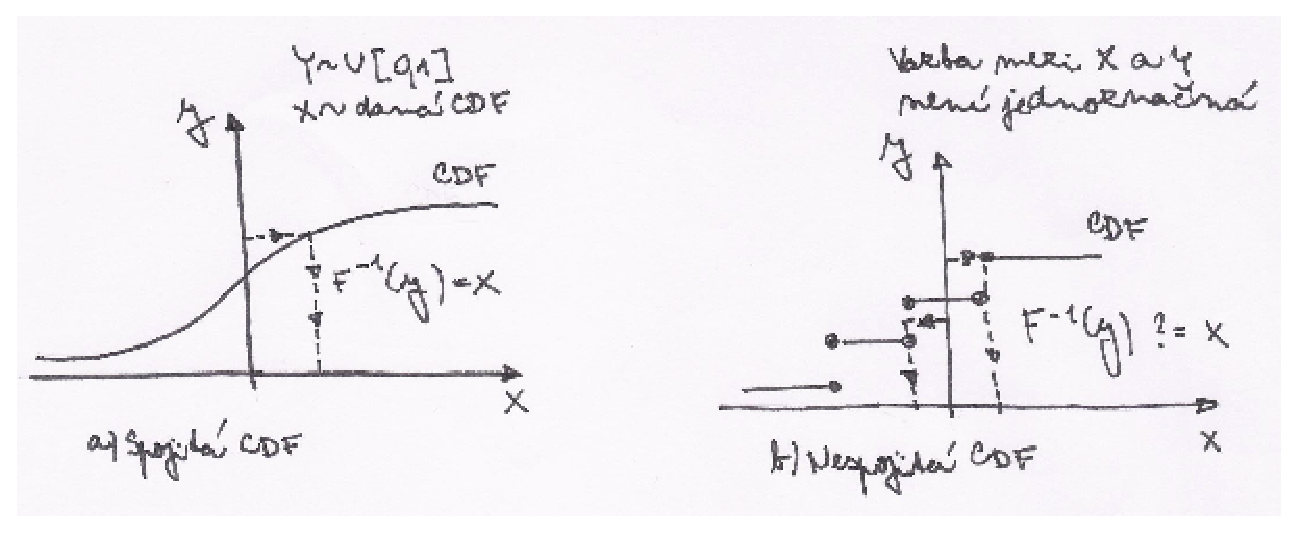
\includegraphics[scale = 0.5]{pictures/inv_cdf.eps}
\caption{Inverze kumulativní distribuční funkce}
\label{inv_cdf}
\end{figure} 

\subsection{Sklarova věta}

Libovolná distribuční funkce definovaná nad $R^d$ v sobě implicitně zahrnuje kopula funkci. Toto tvrzení platí také naopak. Jestliže ``spojíme'' kopula funkci a marginální cdf, získáme vícerozměrné rozdělení. Toto tvrzení vyplývá z následující věty.

\begin{theorem}[Sklarova věta]
Uvažujme $d$-rozměrnou distribuční funkci $F$ s marginálními distribučními funkcemi $F_1, ..., F_d$. Pak existuje kopula funkce taková, že
\begin{equation}
F(x_1, ..., x_d) = C\big(F_1(x_1), ..., F_d(x_d)\big)
\end{equation}
pro všechna $x_i$ v $(-\infty, \infty)$, $i = 1, ..., d$. Jestliže je $F_i$ spojitá pro všechna $i = 1, ..., d$, pak je $C$ jedinečné. V opačném případě je $C$ jedinečné pouze na $Ran(F_1) \times \cdots \times Ran(F_d)$, kde $Ran(F_i)$ označuje obor hodnot distribuční funkce $F_i$\footnote{Např. pro hrací kostku je obor hodnot příslušné distribuční funkce definován jako $\{\frac{1}{6}, \frac{2}{6}, ..., \frac{6}{6}\}$.}.

Výše uvedené tvrzení platí i naopak. Uvažujme kopula funkci $C$ a jednorozměné distribuční funkce $F_1, ..., F_d$. Pak $F$ definovaná dle (1.3) je vícerozměrnou distribuční funkcí s marginálními distribučními funkcemi $F_1, ..., F_d$.
\end{theorem}
S využitím vztahu $F_i \circ F_i^{\leftarrow}(y) \ge y$ získáváme
\begin{equation}
C(u) = F\big(F_1^{\leftarrow}(u_1), ..., F_d^{\leftarrow}(u_d)\big)
\end{equation}
Zatímco (1.3) je zpravidla výchozím bodem pro simulaci, vztah (1.4) slouží spíše pro ``oddělení'' kopula funkce od vícerozměrné distribuční funkce.

\subsection{Hustota pravděpodobnosti kopule}

Dle definice je kopula funkce distribuční funkcí. Vzhledem k obtížné interpretaci kumulativní distribuční funkce se často používá hustota pravděpodobnosti (pdf - probability density function). Je však třeba zmínit, že ne všechny kopula funkce mají odpovídající hustotu pravděpodobnosti. Nicméně má-li kopula funkce diferenci požadovaného řádu, lze hustotu pravděpodobnosti vyjádřit jako
\begin{equation*}
c(u) := \frac{\partial^d C(u_1, ..., u_d)}{\partial u_1, ..., u_d}
\end{equation*}

Jestliže lze kopula funkci vyjádřenou ve tvaru (1.4) derivovat, což má za následek $F_i^{\leftarrow} = F_i^{-1}$, lze odpovídající hustotu pravděpodobnosti vyjádřit jako
\begin{equation*}
c(u) = \frac{f\big(F_1^{-1}(u_1), ..., F_d^{-1}(u_d)\big)}{f_1\big(F_1^{-1}(u_1)\big) \cdots f_d\big(F_d^{-1}(u_d)\big)}
\end{equation*}
kde $f$ označuje sdruženou hustotu pravděpodobnosti a $f_i, i = 1, ..., d$ marginální hustotu pravděpodonosti jednotlivých náhodných veličin.
\begin{proof}
S využitím pravidla pro derivaci složené funkce (chain rule)
\begin{equation*}
\frac{d f(g(x))}{dx} = \frac{df}{dg}\frac{dg}{dx} = f'(g(x))g'(x)
\end{equation*}
a skutečností $F(F^{-1}(u)) = u$ a $\frac{du}{du} = 1$, lze snadno dokázat
\begin{equation*}
\frac{dF(F^{-1}(u))}{du} = f(F^{-1}(u))\frac{dF^{-1}(u)}{du} = 1
\end{equation*}
z čehož vyplývá
\begin{equation*}
\frac{dF^{-1}(u)}{du} = \frac{1}{f(F^{-1}(u))}
\end{equation*}
Derivací dvourozměné kopule funkce ve tvaru (1.4) tak získáme
\begin{multline*}
\frac{dF\big(F_1^{-1}(u_1),F_2^{-2}(u_2)\big)}{du_1du_2} = f\big(F_1^{-1}(u_1), F_2^{-1}(u_2)\big)\frac{F_1^{-1}(u_1)}{du_1}\frac{F_2^{-1}(u_2)}{du_2}\\
= \frac{f\big(F_1^{-1}(u_1), F_2^{-1}(u_2)\big)}{f_1\big(F_1^{-1}(u_1)\big)f_2\big(F_2^{-1}(u_2)\big)}
\end{multline*}
\end{proof}

\subsection{Podmíněné rozdělení}

Uvažujme dvě uniformní náhodné veličiny $U_1$ a $U_2$. Předpokládejme, že známe kopula funkci $C$ a hodnotu náhodné veličiny $U_1$. Cílem je odvodit podmíněné rozdělení, které lze použít pro odhad náhodné veličiny $U_2$. Za předpokladu dostatečné regularity lze odvodit podmíněnou distribuční funkci.
\begin{multline*}
P(U_2 \le u_2 | U_1 = u_1) = \lim_{\delta \rightarrow 0}\frac{P(U_2 \le u_2, U \in (u_1 - \delta, u_1 + \delta])}{P(U_1 \in (u_1 - \delta, u_1 + \delta])}\\
= \lim_{\delta \rightarrow 0}\frac{C(u_1 + \delta, u_2) - C(u_1 - \delta, u_2)}{2 \delta} = \frac{\partial C(u_1, u_2)}{\partial u_1}
\end{multline*}
Podmíněné distribuční funkce lze tedy odvodit derivací kopula funkce $C$ dle $u_1$. Odpovídající podmíněnou hustotu pravděpodobnosti lze získat následnou derivací dle $u_2$.

\subsection{Hraniční hodnoty kopule}

\begin{proposition}
Uvažujme náhodné veličiny $X_1, ..., X_d$, jejichž závislost je definovaná kopula funkcí $C$. Nechť $T_i: R \rightarrow R, i = 1, ..., d$ je striktně rostoucí funkcí. Pak je závislost náhodných veličin $T_1(X_1), ..., T_d(X_d)$ definována toutéž kopula funkcí $C$. 
\end{proposition}
Jinými slovy, striktně rostoucí transformace nemění strukturu závislosti, což se na první podhled může zdát kontraintuitivní. Monotonní transformace totiž sice mění závislost mezi náhodnými veličinami, nicméně po očištění o vliv marginálních distribučních funkcí získáme shodnou strukturu závislosti definovanou kopula funkcí $C$.

Hoeffding a Fréchet nezávisle na sobě odvodili, že kopula funkce vždy leží v rámci určitých hraničních hodnot. Důvody lze nalézt při zkoumání extrémních případů závislosti.
Uvažujme dvě náhodné veličiny $U_1$ a $U_2$. Jestliže $U_1 = U_2$, pak hovoříme o tzv. komonotonických (comonotic) náhodných veličinách a jejich kopula funkce je dána vztahem
\begin{equation}
C(u_1, u_2) = P(U_1 \le u_1, U_1 \le u_2) = min(u_1, u_2)
\end{equation}
Tento typ kopule získéme vždy, když $X_2 = T(X_1)$, kde $T$ je monotonní transformace.
V případě, kdy jsou $U_1$ a $U_2$ nezávislé, je kopula funkce rovna
\begin{equation}
C(u_1, u_2) = u_1 u_2
\end{equation}
Dalším extrémní situací je $U_2 = 1 - U_1$, kdy hovoříme o tzv. kontramonotonických (countermonotonic) náhodných veličinách. Kopula funkce pro $1 - u_2 < u_1$ je
\begin{multline}
C(u_1, u_2) = P(U_1 \le u_1, U_2 \le u_2) = P(U_1 \le u_1, 1 - U_1 \le u_2)\\
= P(U_1 \le u_1, U_1 \ge 1 - u_2) = P(1 - u_2 \le U_1 \le u_1)\\
= u_1 - (1 - u_2) = u_1 + u_2 - 1
\end{multline}
Výše uvedené lze rozšířit na vícerozměrné rozdělení. Ačkoliv komonotonická kopule existuje pro libovolnou dimenzi $d$, kontramonotonická kopule existuje pouze pro $d = 2$\footnote{Uvažujme náhodné veličiny $X_1$, $X_2$ a $X_3$. Jako kontramonotonické zvolme páry $(X_1, X_2)$ a $(X_1, X_3)$. Tato volba představuje omezení pro závislost mezi $X_2$ a $X_3$. Jestliže se $X_1$ sníží, jak $X_2$ tak $X_3$ se musí zvýšit a tudíž nemohou být kontramonotonické.}, nicméně hraniční hodnoty jsou platné i pro vyšší dimenze.

\begin{theorem}[Fréchet-Hoeffdingovy hraniční hodnoty]
Uvažujme kopula funkci $C(u) = C(u_1, ..., u_d)$. Pak platí
\begin{equation*}
\max\left(\sum_{i = 1}^d u_i + 1 - d, 0 \right) \le C(u) \le \min\left(u_1, ..., u_d\right)
\end{equation*}
\end{theorem}

\begin{figure}[htp]
\centering
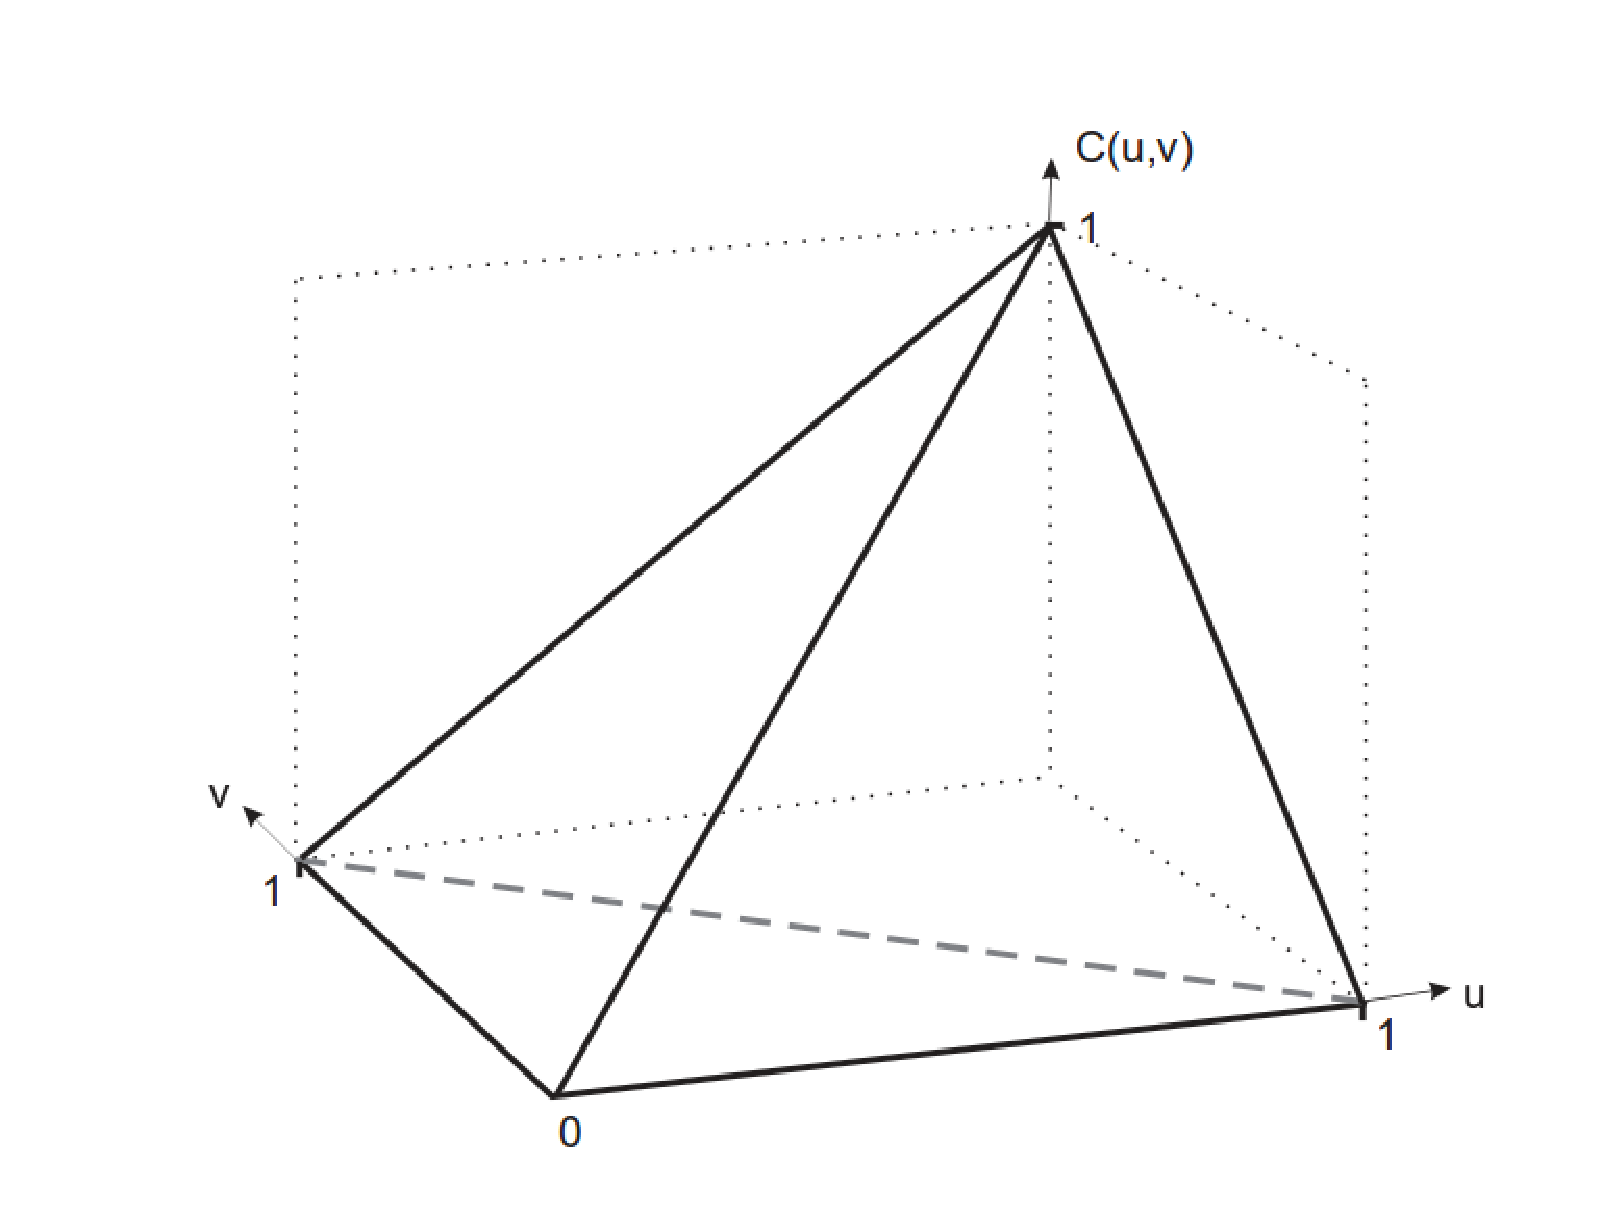
\includegraphics[scale = 0.35]{pictures/copula_boundary.eps}
\caption{Fréchet-Hoeffdingovy hraniční hodnoty - Každá kopula funkce leží uvnitř zobrazené pyramidy. Povrch daný spodní a zadní stěnou pyramidy (dolní hranice) představuje kontramonotonistickou kopula funkcí $C(u, v) = \max\{u + v -1, 0\}$. Povrch daný přední stěnou pyramidy (horní hranice) pak představuje monotonostickou kopula funkci $C(u, v) = \min(u, v)$.}
\label{copula_boundary}
\end{figure} 
